\documentclass[12pt, twoside]{article}
\usepackage[letterpaper, margin=1in, headsep=0.2in]{geometry}
\setlength{\headheight}{0.6in}
%\usepackage[english]{babel}
\usepackage[utf8]{inputenc}
\usepackage{microtype}
\usepackage{amsmath}
\usepackage{amssymb}
%\usepackage{amsfonts}
\usepackage{siunitx} %units in math. eg 20\milli\meter
\usepackage{yhmath} % for arcs, overparenth command
\usepackage{tikz} %graphics
\usetikzlibrary{quotes, angles}
\usepackage{graphicx} %consider setting \graphicspath{{images/}}
\usepackage{parskip} %no paragraph indent
\usepackage{enumitem}
\usepackage{multicol}
\usepackage{venndiagram}

\usepackage{fancyhdr}
\pagestyle{fancy}
\fancyhf{}
\renewcommand{\headrulewidth}{0pt} % disable the underline of the header
\raggedbottom
\hfuzz=2mm %suppresses overfull box warnings

\usepackage{hyperref}

\fancyhead[LE]{\thepage}
\fancyhead[RO]{\thepage \\ Name: \hspace{4cm} \,\\}
\fancyhead[LO]{BECA / Dr. Huson / Geometry\\*  Unit 1: Segments, length, and area\\* 22 Sept 2022}

\begin{document}

\subsubsection*{1.9 Rounding and circle area}
\begin{enumerate}
\item Write these formulas and definitions in your notebook:
  \begin{itemize}
    \item The radius, $r$, is the distance from the center to the edge of a circle. 
    \item The diameter, $D$, is the distance all of the way across a circle, two times the radius. $D=2r$. 
    \item The circumference, $C$, is the distance around the circle (its perimeter).
  \end{itemize}
  \[A=\pi r^2\]
  \[C= 2\pi r\]

\item Given the circle centered at $O$ with radius $r=4$. Leave an exact answer, in terms of $\pi$.
  \begin{multicols}{2}
    \begin{enumerate}
      \item Find the circumference of circle $O$. %\vspace{1cm}
      \item Find the area of the circle.\vspace{2cm}
    \end{enumerate}
    %\columnbreak
    \begin{tikzpicture}[scale=.635]
      \draw[help lines] (-5,-4) grid (5,4);
      \draw (0,0) circle [radius=4] node[below]{$O$};
      \draw[fill] (0,0) circle [radius=0.05];
    \end{tikzpicture}
  \end{multicols}

\item Find the area $A$ of a circle with radius 13 inches to the \emph{nearest square inch}. \vspace{2cm}

\item Given circle $O$ with area $A=64 \pi$ square centimeters. Find the radius, $AB=r$.
\begin{multicols}{2}
  \begin{tikzpicture}[scale=0.8]
    \draw (0,0) circle[radius=3];
    \draw[fill] (0,0) circle [radius=0.08];
    \draw[thick, <->]
      (0:3) node[right]{$B$}--
      (0.1,0) node[left=5pt]{$A$};
    \draw (1.5,0) node[below]{$r=?$};
  \end{tikzpicture} \par
 Start with the formula \par \smallskip
$A = \pi r^2 = 64 \pi$
\end{multicols} \vspace{1cm}

\newpage
\item In mathematics we commonly use the special, irrational number, $\pi = 3.14159265358...$. Mark and label $\pi$ on the number line below.\par \bigskip
\begin{tikzpicture}[scale=3]
  \draw[->] (0,0)--(5.1,0);
  \foreach \x in {0, 0.1,...,5.0}
    \draw[shift={(\x,0)}] (0pt,-1pt)--(0pt,1pt);
  \foreach \x in {0, 0.5,...,5.0}
    \draw[shift={(\x,0)}] (0pt,-3pt)--(0pt,3pt)node[below=20pt]{$\x$};
\end{tikzpicture} \medskip

\item A semicircle is half of a circle, as shown below. The given semicircle has a radius of $r=5$. Round your answers to the \emph{nearest tenth}.
\begin{multicols}{2}
\begin{tikzpicture}[scale=.635]
  \draw[thick, ->] (-1.2,0) -- (8.4,0) node[below right]{$x$};
  \draw[thick, ->] (0,-1.2)--(0,6.4) node[left]{$y$};
  \draw[thick] (1,2)node[below]{$A$} --
    (7,2)node[below]{$B$};
  \draw[thick] (7,2) arc (0:180:3);
  \draw[fill] (4,2) circle [radius=0.08]node[below]{$O$};
  \draw[->, xshift=4cm,yshift=2cm] (0,0)--(30:3);
  \node at (5,3.5){$r=5$};
\end{tikzpicture}
\begin{enumerate}
  \item Find the diameter, $D=AB$. \bigskip
  \item Find the perimeter (the half circumference plus the diameter) \vspace{2.5cm}
  \item Find the area of the semicircle.
\end{enumerate}
\end{multicols} \vspace{3cm}

\item Find the area of the shape shown below composed of a rectangle and semicircular cap. Leave your answer as an exact value in terms of $\pi$.
  \begin{flushright}
  \begin{tikzpicture}[scale=.635]
    \draw[help lines] (-1,-1) grid (7,7);
    \draw[thick, ->] (-1.2,0) -- (7.4,0) node [below right]{$x$};
    \draw[thick, ->] (0,-1.2)--(0,7.4) node [left]{$y$};
    \draw[thick] (1,1)--(5,1)--(5,4)--(1,4)--cycle;
    \draw[thick] (5,4) arc (0:180:2);
  \end{tikzpicture}
  \end{flushright}

\end{enumerate}
\end{document}